\documentclass[
  10pt,     % set default generic font size
  %handout   % ignores all the \pause commands
]{beamer}
\usetheme[block=fill]{metropolis}

% -----------------------------------------------------------------------------
% Title and Author Information -- Need to Edit
% -----------------------------------------------------------------------------

\title{Evaluating staged investments in critical infrastructure for climate adaptation}
\subtitle{Interdisciplinary Ph.D. Workshop in Sustainable Development 2019}
\date{13 April 2019}
\author{\alert{James Doss-Gollin}$^1$, David J. Farnham$^2$, Scott Steinschneider$^3$, Upmanu Lall$^1$}
\institute{
  $^1$Columbia University Department of Earth and Environmental Engineering\\
  $^2$Carnegie Institution for Science\\
  $^3$Department of Biological and Environmental Engineering, Cornell University}
\titlegraphic{\hfill\includegraphics[height=1.25cm]{SeasCrown_blue.png}}


% Add footer for AGU
\setbeamertemplate{footline}[text line]{%
  \parbox{0.8\linewidth}{
    \vspace*{-8pt}James Doss-Gollin (\url{james.doss-gollin@columbia.edu})
  }
  \hfill%
  \parbox{0.15\linewidth}{
    \vspace*{-8pt}\raggedleft\insertframenumber
  }
}

% -----------------------------------------------------------------------------
% Package Configuration -- Don't Necessarily Need to Edit
% -----------------------------------------------------------------------------

% Packages with Options
\usepackage[english]{babel}

% Package List
\usepackage{
  amsmath,amssymb,                    % for more math commands
  array,                              % for custom table widths
  appendixnumberbeamer,               % don't count appendix slides in progress bar
  booktabs,                           % for better (alternative?) tables
	physics,                            % for better notation
  siunitx,                            % for SI notation
}

% cool fonts
\usepackage{fontspec}
\usepackage{fontawesome5}

% figures
\usepackage{graphicx}
\graphicspath{{../fig/}} % can add more

% Fixed-width columns
\usepackage{array}
\newcolumntype{L}[1]{>{\raggedright\let\newline\\\arraybackslash\hspace{0pt}}m{#1}}

% Change the captions
\setbeamerfont{caption}{size=\scriptsize}

% macros
\usepackage{xspace}
\newcommand*{\eg}{e.g.\@\xspace}
\newcommand*{\ie}{i.e.\@\xspace}
\makeatletter
\newcommand*{\etc}{%
    \@ifnextchar{.}%
        {etc}%
        {etc.\@\xspace}%
}
\makeatother
\newcommand{\usd}[1]{\SI[round-precision=2,round-mode=places,round-integer-to-decimal]{#1}[\$]{}}
\newcommand{\normal}{\mathcal{N}}
\newcommand*{\ditto}{---''---}

% Biblatex Setup using a file called library.bib
\setbeamertemplate{bibliography item}[text] % don't print the symbols

\usepackage[
  backend=biber,
  doi=true,
  url=false,
  isbn=false,
  style=authoryear-comp, natbib=true,
  backref=false,
  maxbibnames=3,
  maxcitenames=2,
  uniquename=false,
  uniquelist=false
]{biblatex}
\renewbibmacro{in:}{}
\AtEveryBibitem{\clearfield{month}\clearfield{pages}}
\addbibresource{library.bib}

% Use the glossaries package
\usepackage[acronym]{glossaries}
\makeglossaries
\newacronym{acc}{ACC}{anthropogenic climate change}
\newacronym{amo}{AMO}{Atlantic Multidecadal Oscillation}
\newacronym{cba}{CBA}{Cost-Benefit Analysis}
\newacronym{enso}{ENSO}{the El Ni\~{n}o-Southern Oscillation}
\newacronym{ffa}{FFA}{flood frequency analysis}
\newacronym{gcm}{GCM}{general circulation model}
\newacronym{hmm}{HMM}{Hidden Markov Model}
\newacronym{iid}{IID}{independent and identically distributed}
\newacronym{ipcc}{IPCC}{International Panel on Climate Change}
\newacronym{ipo}{IPO}{Interdecadal Pacific Oscillation}
\newacronym{lbda}{LBDA}{living blended drought analysis}
\newacronym{lfv}{LFV}{low-frequency climate variability}
\newacronym{nao}{NAO}{North Atlantic Oscillation}
\newacronym{npv}{NPV}{Net Present Value}
\newacronym{pdo}{PDO}{Pacific Decadal Oscillation}
\newacronym{s2d}{S2D}{seasonal to decadal}
\newacronym{s2s}{S2S}{sub-seasonal to seasonal}

% this has to come last
\usepackage{cleveref}
\usepackage{hyperref}

% -----------------------------------------------------------------------------
% BEGIN DOCUMENT HERE
% -----------------------------------------------------------------------------

\begin{document}

% TITLE PAGE
\maketitle

\begin{frame}{The really big picture}
  \begin{figure}
    \centering
    \pause
    \includegraphics[height=0.325\textheight]{powerless.png}~
    \includegraphics[height=0.325\textheight]{ho-2017-1.png}\\
    \pause
    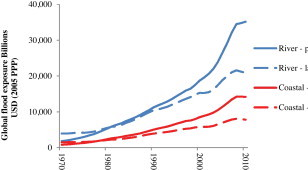
\includegraphics[height=0.325\textheight]{jongman-fig-2.jpg}~
    \includegraphics[height=0.325\textheight]{wapo-usa-temp.png}
  \end{figure}
  \citep{economist-nigeria:2016,Ho:2017gy,Jongman:2012cr}
\end{frame}

\begin{frame}{Motivating case study}
  What to do after Sandy? \citep{CityofNewYork:2013uh}
  \begin{figure}
    \centering
    \includegraphics[height=0.35\textheight]{three-barriers.png}~
    \includegraphics[height=0.35\textheight]{dull-disasters.png}\\
    \includegraphics[height=0.3\textheight]{flood-concept.png}~
    \includegraphics[height=0.3\textheight]{coastal-resiliency.png}
  \end{figure}
\end{frame}

\begin{frame}{Today}
  My perspective: sequential planning under uncertainty
  \pause
  \begin{enumerate}
    \item How does organized variability in the climate inform this planning?
    \pause
    \item Observations $\Rightarrow$ notice three interesting things about the world
    \pause
    \item Stylized computational experiments $\Rightarrow$ understand implications in an idealized system
  \end{enumerate}
  \pause
  Paper submitted to Earth's Future; all codes are available at \url{http://github.com/jdossgollin/2018-robust-adaptation-cyclical-risk}
\end{frame}

\section{Hypotheses}

\begin{frame}{Idea 1: Risk Estimates over Finite Future Periods}
  \begin{alertblock}{Typical Approach:}
    \acrfull{cba}, probably with discounting, over a \alert{finite} planning horizon of $M$ years.
  \end{alertblock}
  \pause
  Project success depends on climate conditions over this finite planning period:
  \begin{itemize}
    \item For dam, storm barrier: $M \geq \SI{50}{years}$
    \item For cat bond, zoning change: $M \leq \SI{5}{years}$
  \end{itemize}
  \pause
  Small $M$: defer large investment and allow some uncertainties to be resolved
\end{frame}

\begin{frame}{Idea 2: Hydroclimate Systems Vary on Many Scales}
  Inter-annual to multi-decadal cyclical variability key (for small $M$)
  \begin{figure}
    \centering
    \includegraphics[width=\textwidth,height=0.55\textheight,keepaspectratio=true]{observed-lfv.pdf}
    \caption{
      (a) \SI{500}{year} reconstruction of summer rainfall over Arizona from LBDA \citep{Cook:2010bz}.
      (b) A \SI{100}{year} record of annual-maximum streamflows for the American River at Folsom.
      (c),(d): wavelet global (average) spectra.
    }\label{fig:observed-lfv}
  \end{figure}
\end{frame}

\begin{frame}{Idea 3: Physical Drivers of Risk Depend on $M$}
  The physical drivers of hazard depend on the projection horizon ($M$),
  \begin{figure}
    \centering
    \includegraphics[width=0.7\textwidth,keepaspectratio=true]{conceptual-sketch-a.png}\\
  \end{figure}
  \pause
  but our ability to identify these mechanisms depends on information available (\eg, the length of an $N$-year observational record).
  \begin{figure}
    \centering
    \includegraphics[width=0.7\textwidth,keepaspectratio=true]{conceptual-sketch-b.png}
  \end{figure}
\end{frame}

\section{Stylized Experiments}

\begin{frame}{Experiment Setup}
  \begin{alertblock}{Research Objective}
    How well can one identify \& predict cyclical and secular climate signals over a finite planning period ($M$),  given limited information?
 \end{alertblock}
  Let $P^* = \mathbb{P} \qty(X > X^*)$.
  \pause
  We consider
  \begin{itemize}
    \item 3 \alert{idealized scenarios of climate change}
    \item 3 \alert{simple} models for projecting risk
  \end{itemize}
  Measure bias and variance of $P^*$.
  \vfill
  \pause
  \emph{Don't use these models for actual estimation!}
\end{frame}

\begin{frame}{How it works}
  \begin{figure}
    \centering
    \includegraphics[width=\textwidth,height=0.7\textheight]{Example-NINO3-M100-N50.pdf}
  \end{figure}
\end{frame}

\begin{frame}{Stationary Scenario (LFV Only)}
  \emph{With limited data, the uncertainties caused by extrapolating from complex models lead to poor performance.}
  \begin{figure}
    \centering
    \includegraphics[width=\textwidth,height=0.625\textheight,keepaspectratio=true]{lfv-only-nino3-bias-variance.pdf}
  \end{figure}
\end{frame}

\begin{frame}{Nonstationary Scenario I (Secular Change Only)}
  \emph{Long planning periods need trend estimation, but this demands lots of information.
  For short planning periods, simple models may be better.}
  \begin{figure}
    \centering
    \includegraphics[width=\textwidth,height=0.625\textheight,keepaspectratio=true]{secular-only-nino3-bias-variance.pdf}
  \end{figure}
\end{frame}

\begin{frame}{Nonstationary Scenario II (Secular Change + LFV)}
  \emph{As the system becomes more complex, more data is needed to understand it.}
  \begin{figure}
    \centering
    \includegraphics[width=\textwidth,height=0.625\textheight,keepaspectratio=true]{lfv-secular-nino3-bias-variance.pdf}
  \end{figure}
\end{frame}

\section{Discussion}

\begin{frame}{Summary}
  \begin{columns}[T]
    \begin{column}{0.45\textwidth}
      \begin{itemize}
        \item Investment evaluation depends on climate condition over finite planning period
        \item Physical hydroclimate systems vary on many scales
        \item Physical drivers of risk depend on planning period
      \end{itemize}    
    \end{column}
    \begin{column}{0.55\textwidth}
      \begin{figure}
        \includegraphics[width=\textwidth]{M-N-Sketch.pdf}
      \end{figure}
    \end{column}
  \end{columns}
\end{frame}

\begin{frame}{Conclusions}
  \begin{itemize}
    \item Quasi-periodic and secular climate signals, with different identifiability and predictability, control future uncertainty and risk
    \pause
    \item Adaptation strategies need to consider how uncertainties in risk projections influence success of decision pathways
    \pause
    \item Stylized experiments reveal how bias and variance of climate risk projections influence risk mitigation over a finite planning period
  \end{itemize}
\end{frame}

\section{Next steps}

% -----------------------------------------------------------------------------
% QUESTIONS, BIBLIOGRAPHY
% -----------------------------------------------------------------------------

\renewcommand*{\bibfont}{\small}
\begin{frame}[allowframebreaks]{References}
  \printbibliography[heading=none]
\end{frame}

\begin{frame}[standout]
  \alert{Thanks for your attention!}\\
  \vspace{1.5cm}
  Interested in making these ideas more concrete?
  I'd love to collaborate!\\
  \vspace{1.5cm}
  \begin{tabular}{rl}
    \faIcon[regular]{twitter},\faIcon[regular]{github} & \href{https://twitter.com/jdossgollin}{@jdossgollin} \\
    \faIcon[regular]{envelope} & \href{mailto:james.doss-gollin@columbia.edu}{james.doss-gollin@columbia.edu}\\
    \faIcon[regular]{paperclip} & \url{www.jamesdossgollin.me}
  \end{tabular}
\end{frame}

% -----------------------------------------------------------------------------
% BACKUP SLIDES
% -----------------------------------------------------------------------------

\appendix
\renewcommand{\thefigure}{A\arabic{figure}}
\setcounter{figure}{0}
\renewcommand{\theequation}{A\arabic{equation}}
\setcounter{equation}{0}
\renewcommand{\thetable}{A\arabic{table}}
\setcounter{table}{0}

\section{Supplemental Discussion}

\begin{frame}{Idealized Experiments $\iff$ Real World}
  The idealized models used here are analogs:
  \begin{table}
    \centering
    \begin{tabular}{L{0.425\textwidth}L{0.525\textwidth}}
      \toprule
      Analysis & Real World \\\midrule
      $N$-year record & Total informational uncertainty of an estimate \\\midrule
      Statistical models of increasing complexity and \# parameters & Statistical and dynamical model chains of increasing complexity and \# parameters \\\midrule
      Linear trends & Secular changes of unknown form \\\midrule
      \gls{lfv} from \gls{enso} & \gls{lfv} from many sources \\\midrule
      \gls{lfv} and trend additive & \gls{lfv} and trend interact \\
      \bottomrule
    \end{tabular}
  \end{table}
\end{frame}

\section{Generating Synthetic Streamflow Sequences}

\begin{frame}{Equations for Synthetic Streamflow Generation}
  First
  \begin{equation} \label{eq:lognormal}
    \log Q(t) \sim \normal \qty(\mu(t), \sigma(t)).
  \end{equation}
  Where $\sigma(t) = \xi \mu(t)$, with $\sigma(t) \geq \sigma_\text{min} > 0$.
  Then,
  \begin{equation}\label{eq:nino3}
    \mu(t) = \mu_0 + \beta x(t) + \gamma \qty(t - t_0),
  \end{equation}
  and where $x(t)$ is NINO3.4 index from realistic \gls{enso} model \citep{Zebiak:1987cl,Ramesh:2016hf}
\end{frame}

\begin{frame}{Spectrum of \gls{lfv} Used}
  \begin{figure}
    \includegraphics[width=\textwidth,height=0.6\textheight,keepaspectratio=true]{enso_wavelet}
    \caption{
      Wavelet spectrum of (sub-set of) \gls{enso} model used to embed synthetic streamflow sequences with low-frequency variability.
      \gls{enso} data from \citet{Ramesh:2016hf}.
    }
  \end{figure}
\end{frame}

\section{Climate Risk Estimation}

\begin{frame}{Stationary LN2 Model}
  Treat the $N$ historical observations as \gls{iid} draws from stationary distribution
  \begin{align}\label{eq:ln2-stationary}
    \begin{split}
      \log Q_\text{hist} & \sim \normal \qty(\mu, \ \sigma) \\
      \mu &\sim \normal \qty(7, 1.5) \\
      \sigma &\sim \normal^+ \qty(1, 1)
    \end{split}
  \end{align}
  where $\normal$ denotes the normal distribution and $\normal^+$ denotes a half-normal distribution.
  Fit in Bayesian framework using stan \citep{Carpenter:2017ke}.
\end{frame}

\begin{frame}{Trend LN2 Model}
  Treat the $N$ historical observations as \gls{iid} draws from log-normal distribution with linear trend
  \begin{align}\label{eq:ln2-trend}
    \begin{split}
      \mu &= \mu_0 + \beta_\mu \qty(t - t_0) \\
    \log Q_\text{hist} & \sim \normal \qty(\mu, \ \xi \mu) \\
    \mu_0 & \sim \normal \qty(7, 1.5) \\
    \beta_\mu & \sim \normal \qty(0, 0.1) \\
    \log \xi & \sim \normal \qty(0.1, 0.1)
    \end{split}
  \end{align}
  where $\xi$ is an estimated coefficient of variation.
  Also fit in stan.
\end{frame}

\begin{frame}{Hidden Markov Model}
  Two-state \gls{hmm} \citep[see][]{Rabiner:1986jk} implemented using pomegranate python package \citep{schreiber:2017}.
  See package documentation for reference.
\end{frame}

\end{document}
